\chapter{Implementation}
\label{chapter:implementation}


This chapter describes implementing the framework, as well as its first scene: an outdoors rail track segmentation task. The Dash Cam TODO REF and Drone Cam TODO OREF video datasets are used as inspiration for designing details in the rail tracks and backgrounds, as seen in Figure \ref{fig:ml-pics}. The use of the generator together with a Machine Learning Model is discussed in the next chapter, Section \ref{sec:evaluate-ml}.

The 3D objects that the segmentation task is focused on, in this case the rail tracks and immediate area, are created using procedurally generated graphics. This ensures a great degree of variation and customization for the same object: one can randomize physical properties of each component of the object, such as changing the shape or material of the railroad ties, or randomly skipping missing planks or changing their distance. 


% ###############################################################
\section{Modifying Kubric to use Blender version 3.2}
\label{sec:upgrading-kubric}

The procedurally generated graphics pipeline is implemented in Blender as a feature called "Geometry Nodes". It is a visual and node-based programming environment that allows 3D artists to create and manipulate different attributes of an object's geometry. Operations on geometry made in this way include arithmetic and vector math, conditional logic, curve resampling, mesh triangulation, material selection, ray tracing and object instancing.

The "Geometry Nodes" feature was added in Blender 2.92\footnote{\url{https://wiki.blender.org/wiki/Reference/Release_Notes/2.92/Geometry_Nodes}}, reworked in Blender 3.0 to make designing Geometry Node Groups more abstract and functional\footnote{\url{https://wiki.blender.org/wiki/Reference/Release_Notes/3.0/Nodes_Physics}}. Later releases have added more node types and performance improvements\footnote{\url{https://wiki.blender.org/wiki/Reference/Release_Notes/3.1/Nodes_Physics}}. We chose to make use of Blender version 3.2\footnote{\url{https://wiki.blender.org/wiki/Reference/Release_Notes/3.2/Nodes_Physics}} as the render engine. This requires updating the Kubric build process and resolving any breaking changes, since at the time of writing, Kubric uses Blender version 2.93.

The upgrade process begins with simple changes: the Python language version was upgraded to 3.10, so the base operating system for the image is increased to a newer version that packages it. Then, the Blender version is switched as mentioned above. These changes are outlined in Listing \ref{fig:idocker-build-diff}.

\begin{figure}[H]
\begin{lstlisting}[language=diff]
--- a/docker/Blender.Dockerfile
+++ b/docker/Blender.Dockerfile
@@ -13,7 +13,7 @@
- FROM ubuntu:20.04 as build
+ FROM ubuntu:21.10 as build

@@ -41,7 +41,7 @@  # RUN git clone https://git.blender.org/blender.git
- RUN git clone https://github.com/blender/blender.git --branch blender-v2.93-release --depth 1
+ RUN git clone https://github.com/blender/blender.git --branch blender-v3.2-release --depth 1 blender
\end{lstlisting}
\caption{Start of the Blender Version Upgrade }
\label{fig:idocker-build-diff}
\end{figure}

Following the changes in Listing \ref{fig:idocker-build-diff}, more adjustments are required for the build process, namely to installed operating system packages, code directories and Python package version numbers. After the build succeeds, more issues follow: Blender function names have changed, and some default behavior has also changed. In total, about 400 lines of code have been added to the Kubric Library to support the new version.

The Docker Build process can also be used for other purposes, such as installing assets or Blender Plugins. An example of Blender Plugin installation is found in Section \ref{sec:dowonload-geo-data}.


% ###############################################################
\section{Saving and Restoring Blender Geometry Nodes}
\label{sec:save-restore-blender-geometry}

In the previous section of this chapter, we discussed how the "Geometry Nodes" feature in Blender is new and actively developed. This means some operations cannot be yet achieved in a straight-forward fashion. This includes saving, restoring and transferring Geometry Nodes between Blender scenes.

In Blender 3.2 there is no direct way to import Geometry Node objects from another Blender project. However, imported Blender objects will keep all their linked Geometry Nodes objects, and all the Materials and Node Groups that are recursively linked by the first-order objects. This feature can be exploited to save and restore "Geomtry Node Groups", the building blocks of this system, by using a dummy object to store the geometry.

TODO code extract for save/restore geometry

This logic is used in the project for incremental "Geometry Node Group" development: the user can open the Blender Geometry Node editor, make changes, save the file, and re-run the save/restore script to use the new version in the scene generation in the full scene.

TODO simple diagram with edit-save-restore-recreate loop


% ###############################################################
\section{Downloading Geographic Data}
\label{sec:dowonload-geo-data}

As stated in the previous chapter, the first stage of the pipeline is concerned with collecting all geographic data required for a 3D scene at a chosen geographic location. To aid in accessing public data from GIS services, we use the freely available BlenderGIS Plugin \footnote{\url{https://github.com/domlysz/BlenderGIS}}.

After the plugin is installed into Blender, it can be used to manually download all required data using the provided User Interface. An example of the manual download flow is available in Figure \ref{fig:manual-download-geo}.

\begin{figure}[H]
\begin{tabular}{ccc}

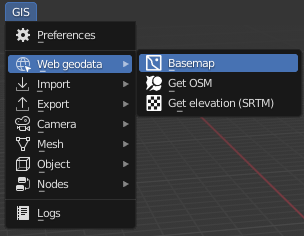
\includegraphics[width=43mm]{src/img/manual-download/1-get-basemap.png} &
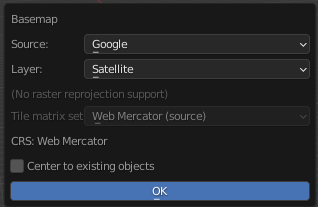
\includegraphics[width=43mm]{src/img/manual-download/2-choose-sat.png} &
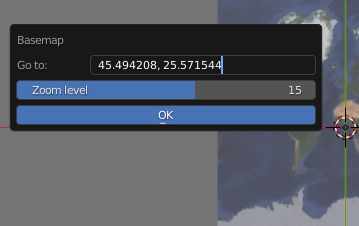
\includegraphics[width=43mm]{src/img/manual-download/3-choose-gps-zoom.png} \\
  (a) Open Base Map Form &  
  (b) Choose Satellite Provider &   
  (c) Choose Location and Zoom \\
  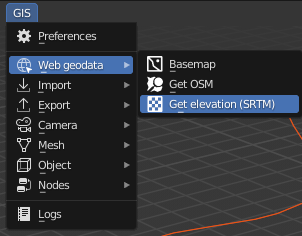
\includegraphics[width=43mm]{src/img/manual-download/4-get-alt.png} &
  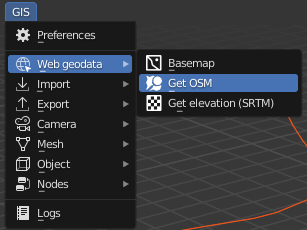
\includegraphics[width=43mm]{src/img/manual-download/5-get-osm.png} &
  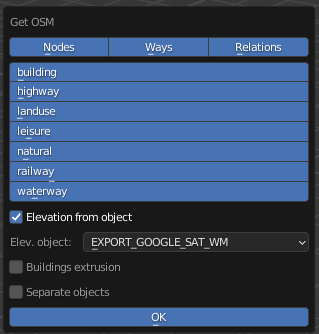
\includegraphics[width=43mm]{src/img/manual-download/6-osm-settings.png} \\
  (d) Obtain Altitude Data &   
  (e) Open OSM Form &          
  (f) Choose OSM Data \\
  \multicolumn{3}{c}{ 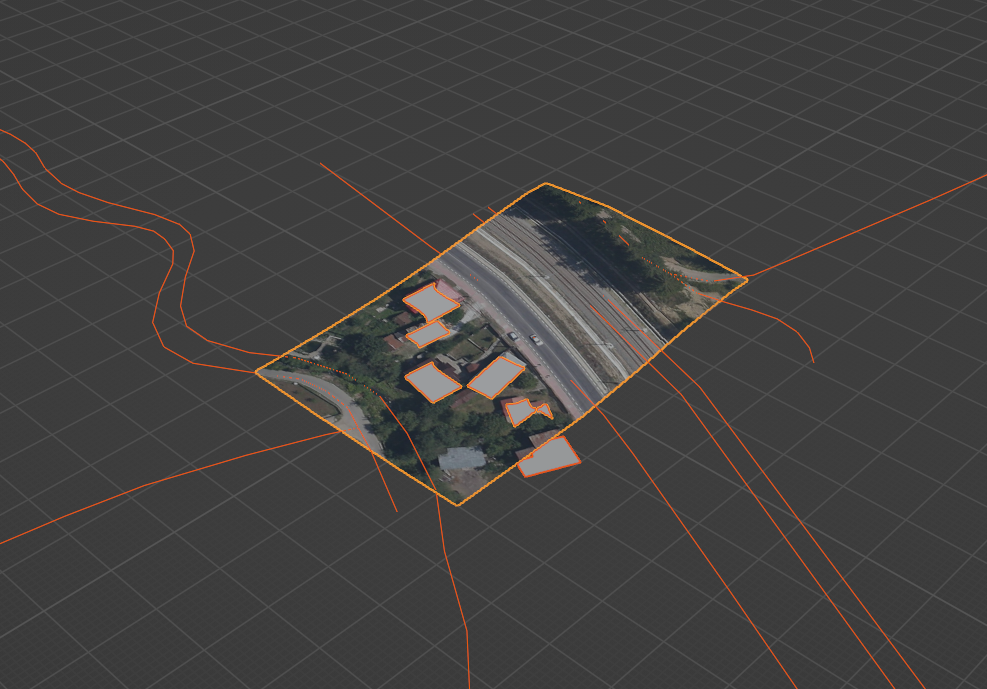
\includegraphics[width=130mm]{src/img/manual-download/7-end-result.png} }  \\ 
  \multicolumn{3}{c}{ (g) Save End Result }
 
\end{tabular}
\caption{Manual Process for Downloading Geographical Data}
\label{fig:manual-download-geo}
\end{figure}


The plugin is also installed in the Docker image at the standard location \texttt{scripts/addons} inside the Blender installation directory. Then, some Python code is executed at module load time to load it and configure its settings. In the example in Listing \ref{fig:blender-plugin}, we show loading and configuring the plugin with the required keys to access the data.

\begin{figure}[H]
\begin{lstlisting}[language=python]
def load_gis_addon():                                   
    bpy.ops.preferences.addon_enable(module='BlenderGIS')
    api_key = os.getenv('SRTM_API_KEY')
    if 'API_Key' not in bpy.context.preferences.addons['BlenderGIS'].preferences.demServer:
        bpy.context.preferences.addons['BlenderGIS'].preferences.demServer += f"&API_Key={api_key}"
    bpy.ops.wm.save_userpref() 
\end{lstlisting}
\caption{Activating and Configuring a Blender Plugin}
\label{fig:blender-plugin}
\end{figure}

The plugin code can then be called from a Blender Operator to ensure its correct execution context, as described by the project maintainer \footnote{\url{https://github.com/domlysz/BlenderGIS/issues/430}}. However, the steps for automating this feature were not implemented in this project, and all data used for this work have been obtained manually through the process in Figure \ref{fig:manual-download-geo}.

% ###############################################################
\section{Combining Levels of Detail}
\label{sec:combine-levels-of-detail}

\begin{figure}[H]
    \centering
    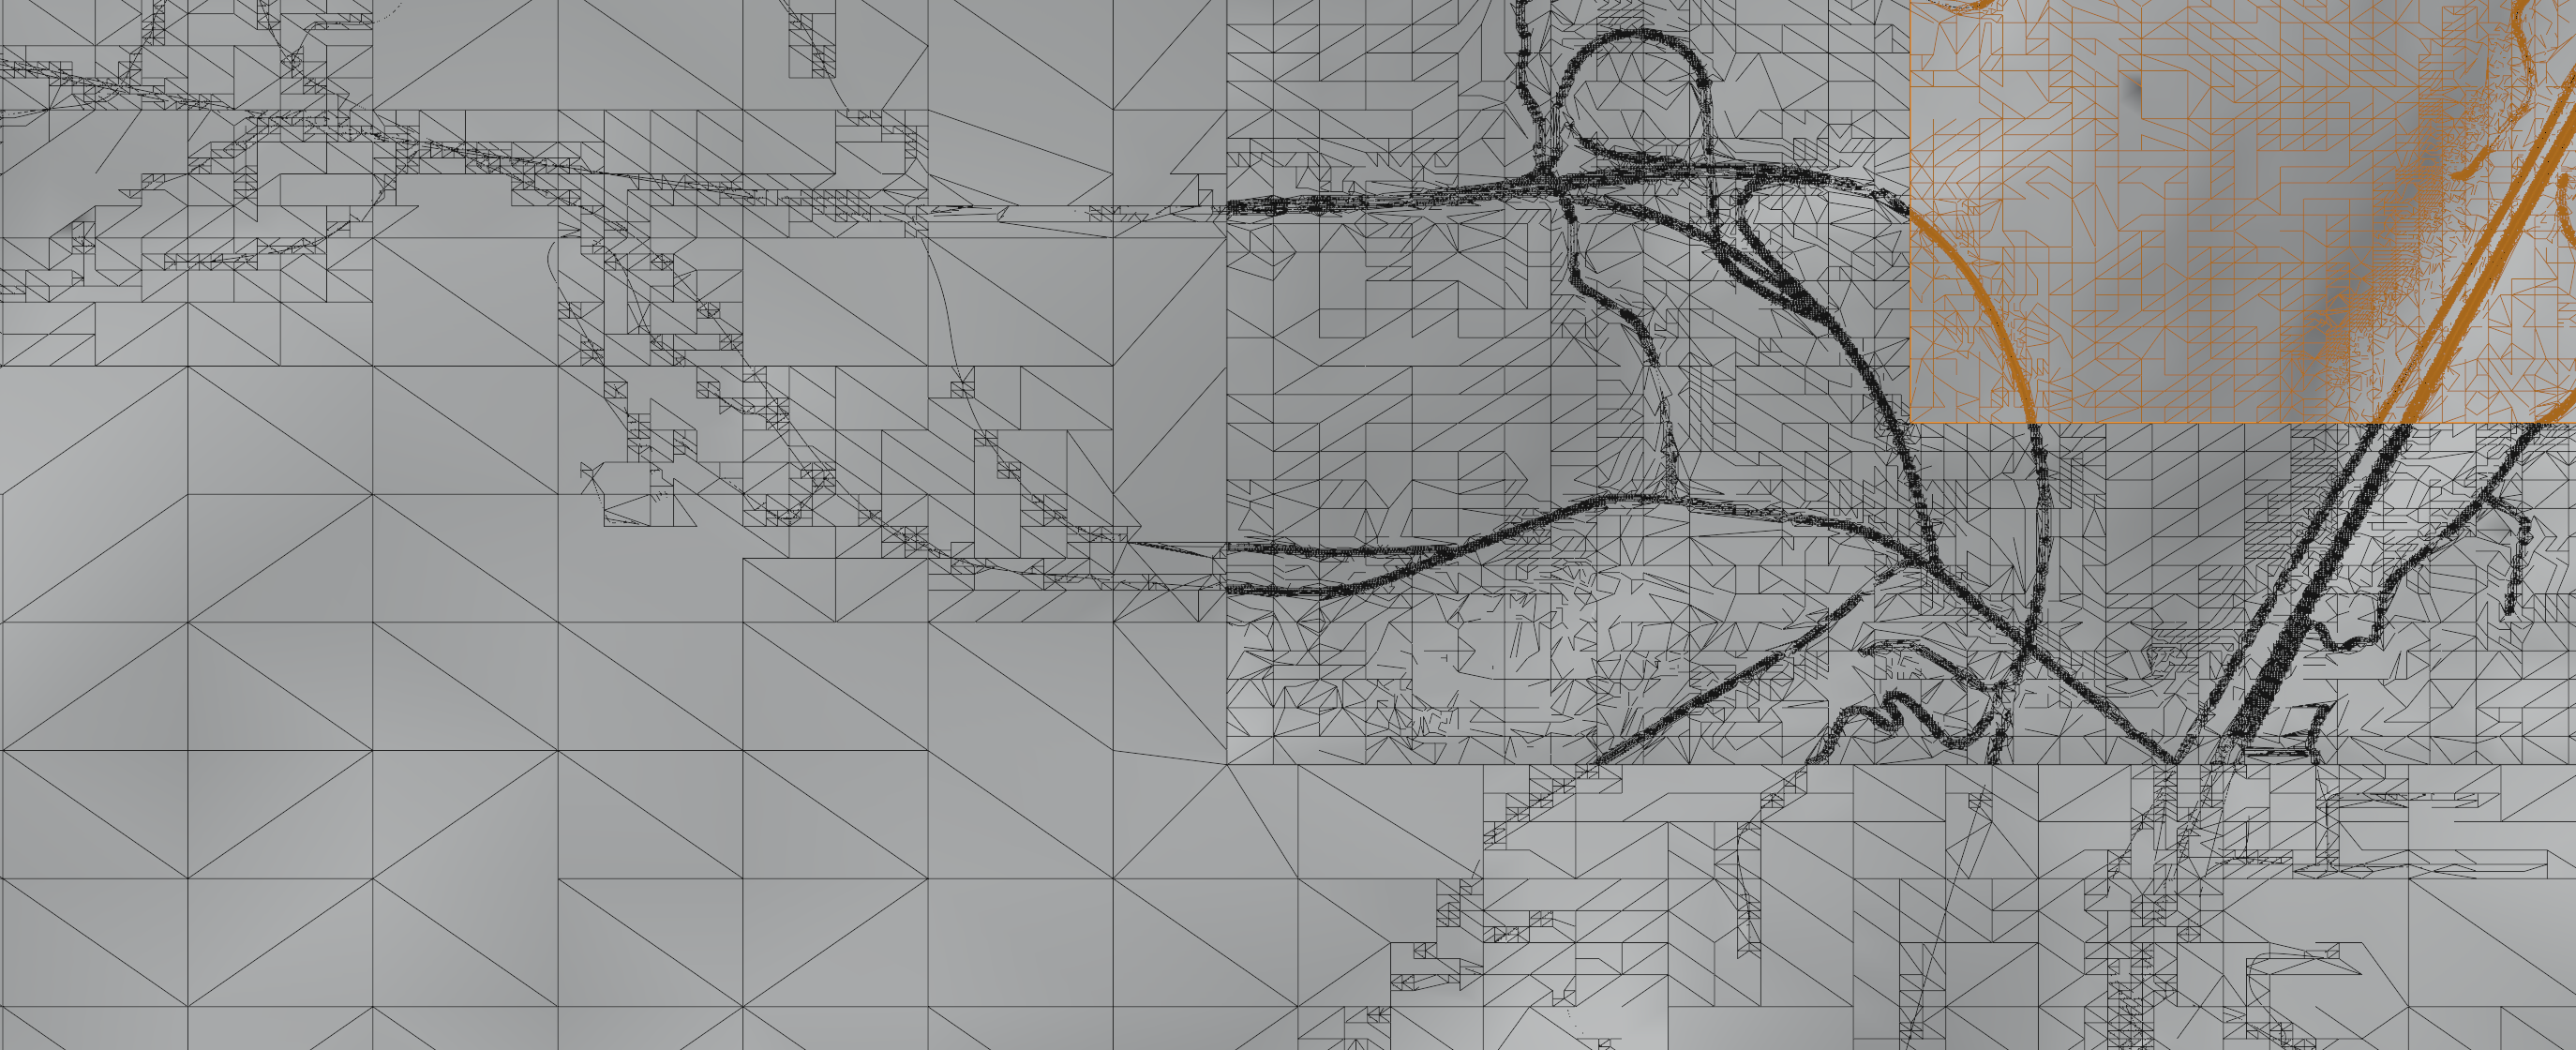
\includegraphics[width=14.5cm]{src/img/pic/pic-1 blender screenshot sat levels of detail.png}
    \caption{Different Levels of Detail }
    \label{fig:impl-levels-of-detail}
\end{figure}

The geographic data aggregated by the BlenderGIS Plugin is stored in a number of Blender files, one for every zoom level. These assets must be combined into a single terrain object, with the scene action happening at the center of the smallest tile.

In addition to the reconciliation of the different level of details for the same terrain, this step must also reconcile the different types of data obtained from different sources. For example, the SRTM height map information does not perfectly match the road position at every point. To resolve this, a height adjustment step is made on both objects: the road track is wrapped to the terrain on the Z axis, and the terrain is flattened in the area immediately around the road track. A similar computation is made in parallel for all the other assets: rail tracks, urban zones, and building perimeters.

Finally, this step ensures adequate tessellation of the ground object. More detailed polygons are generated in the areas immediately around the roads, rails and buildings, and less accurate geometry is used everywhere else. This helps keep the memory footprint low.

\begin{figure}[H]
    \centering
    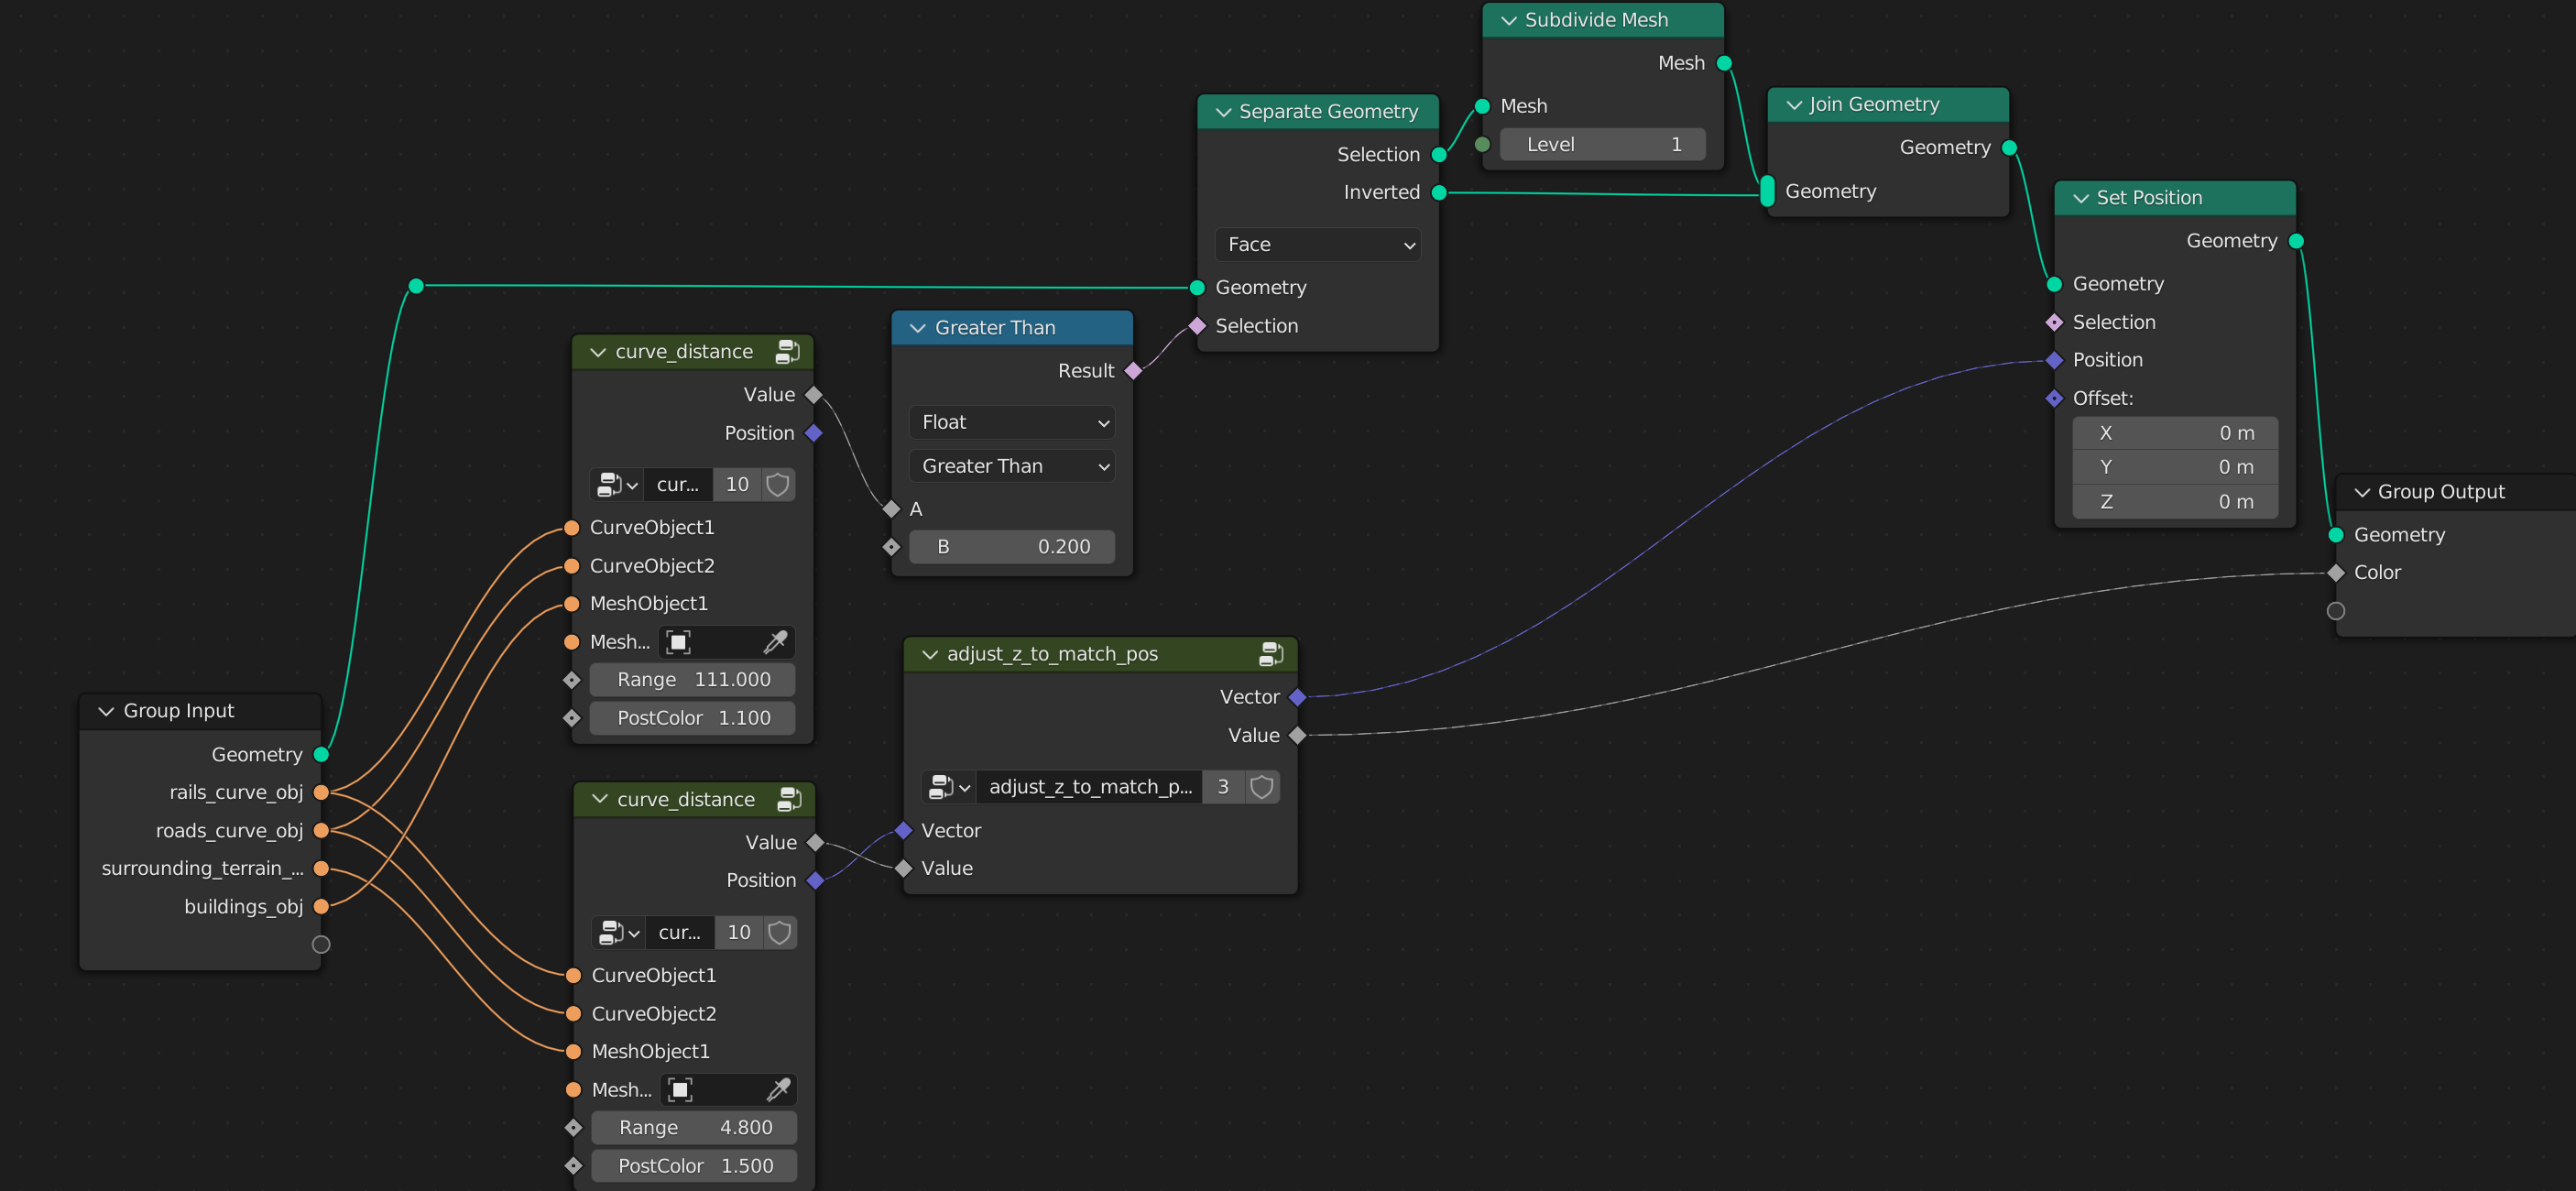
\includegraphics[width=14.5cm]{src/img/pic/pic-2 screenshot of blender adjust terrain geometry node.png}
    \caption{Geometry Node Implementation for Terrain Height Adjustment and Tessellation}
    \label{fig:impl-geom-nodes-terrain}
\end{figure}


The terrain adjustment and tessellation is implemented as a "Geometry Node Group", shown in Figure \ref{fig:impl-geom-nodes-terrain}. It makes use of several subgroups: one for computing distance to a set of curves and meshes (Figure \ref{fig:impl-curve-dist}) and another for adjusting the terrain height based on that distance (Figure \ref{fig:impl-adjust-z-to-match-pos}).

The procedural graphics designer can reuse any "Node Groups" as a part of a larger system, which justifies building a public procedural graphics primitive library to use across different projects. The technical method through such a library is managed is described in Section \ref{sec:save-restore-blender-geometry}.

\begin{figure}[H]
    \centering
    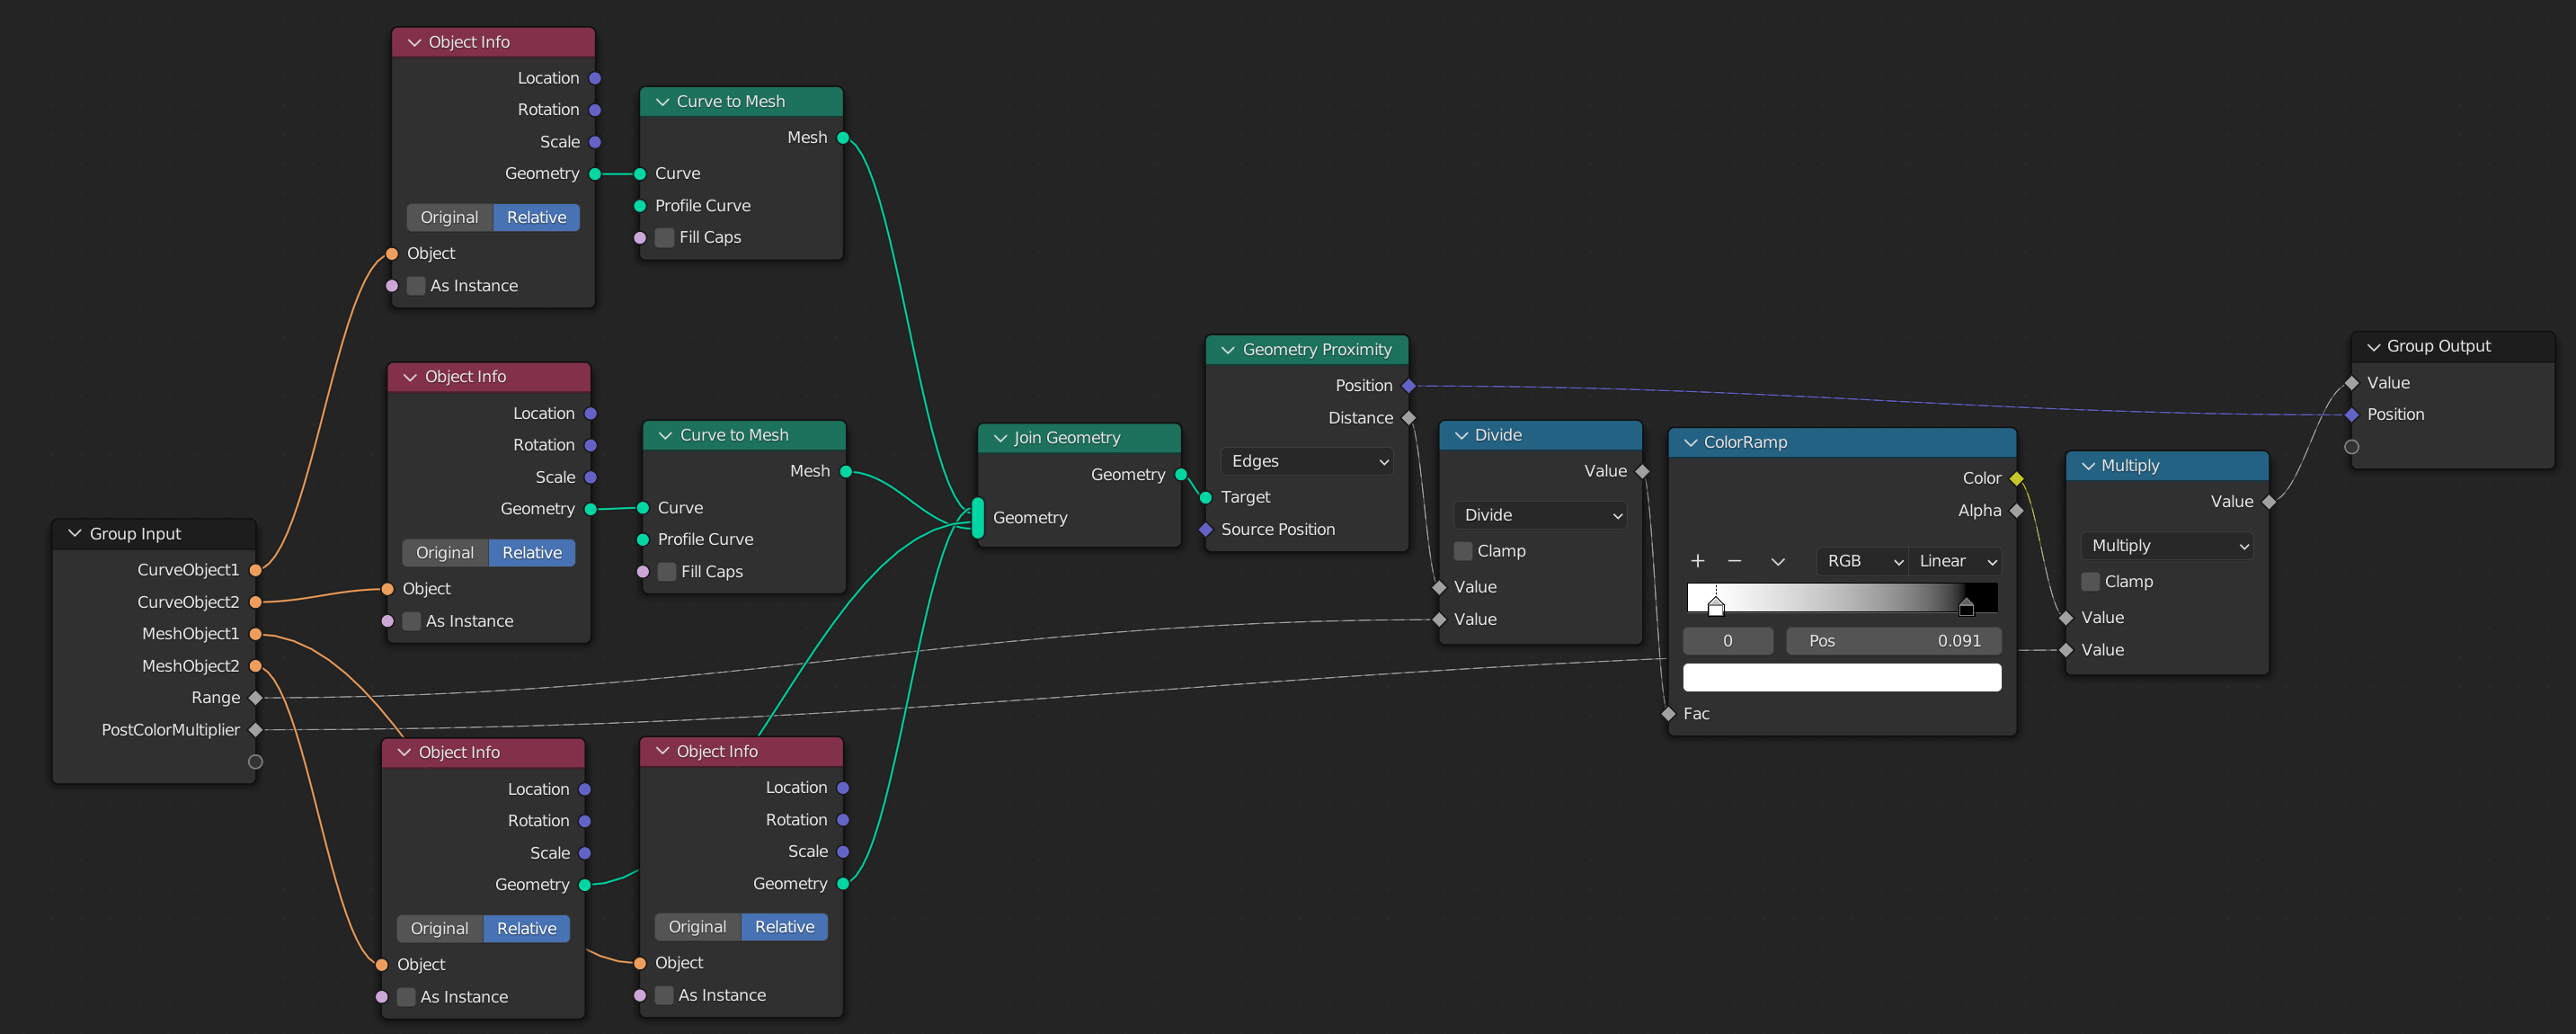
\includegraphics[width=14.5cm]{src/img/pic/pic-3 blender geometry screenshot curve_distance.png}
    \caption{Geometry Node Implementation for Computing Distance to Curves}
    \label{fig:impl-curve-dist}
\end{figure}

During this stage, additional "Geometry Node Groups" are used to create volumes and texture them to represent buildings. Detailed shapes are not implemented, since the scene is primarily concerned with the segmentation of the railway track.

\begin{figure}[H]
    \centering
    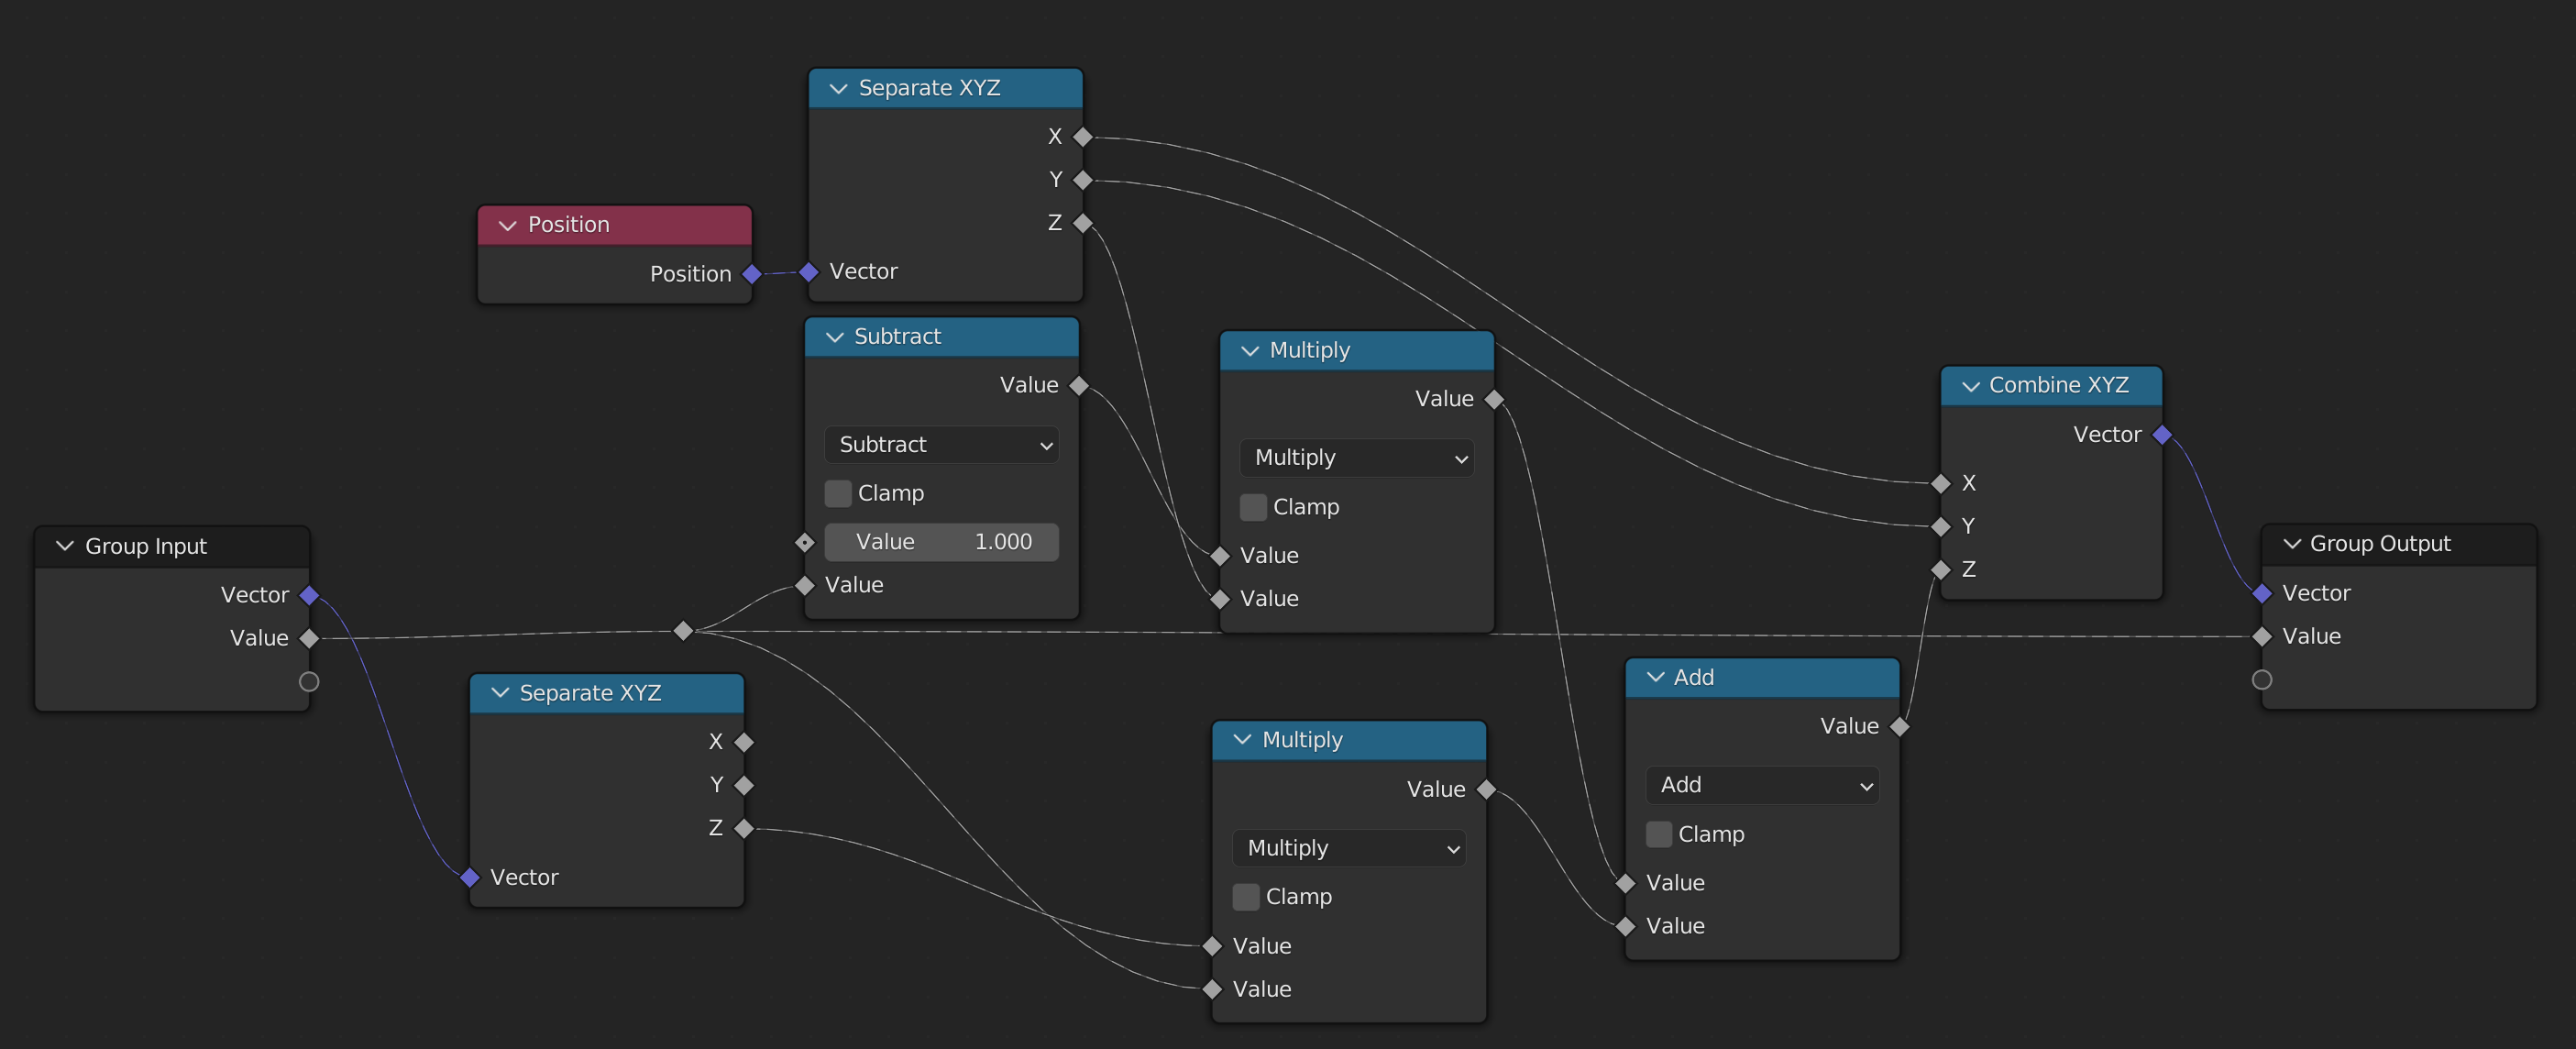
\includegraphics[width=14.5cm]{src/img/pic/pic-4 blender geometry node screenshot adjust_z_to_match_pos.png}
    \caption{Geometry Node Implementation for Adjusting Geometry Height}
    \label{fig:impl-adjust-z-to-match-pos}
\end{figure}

After the ground objects are flattened, adjusted and the different levels of detail are combined, the scene building continues in Section \ref{sec:procedural-railway-generation} with the addition of the foreground object: rail tracks, railroad ties, the fasteners (bolts) and ballast.


% ###############################################################
\section{Procedural Railway Generation}
\label{sec:procedural-railway-generation}


\begin{figure}[H]
    \centering
    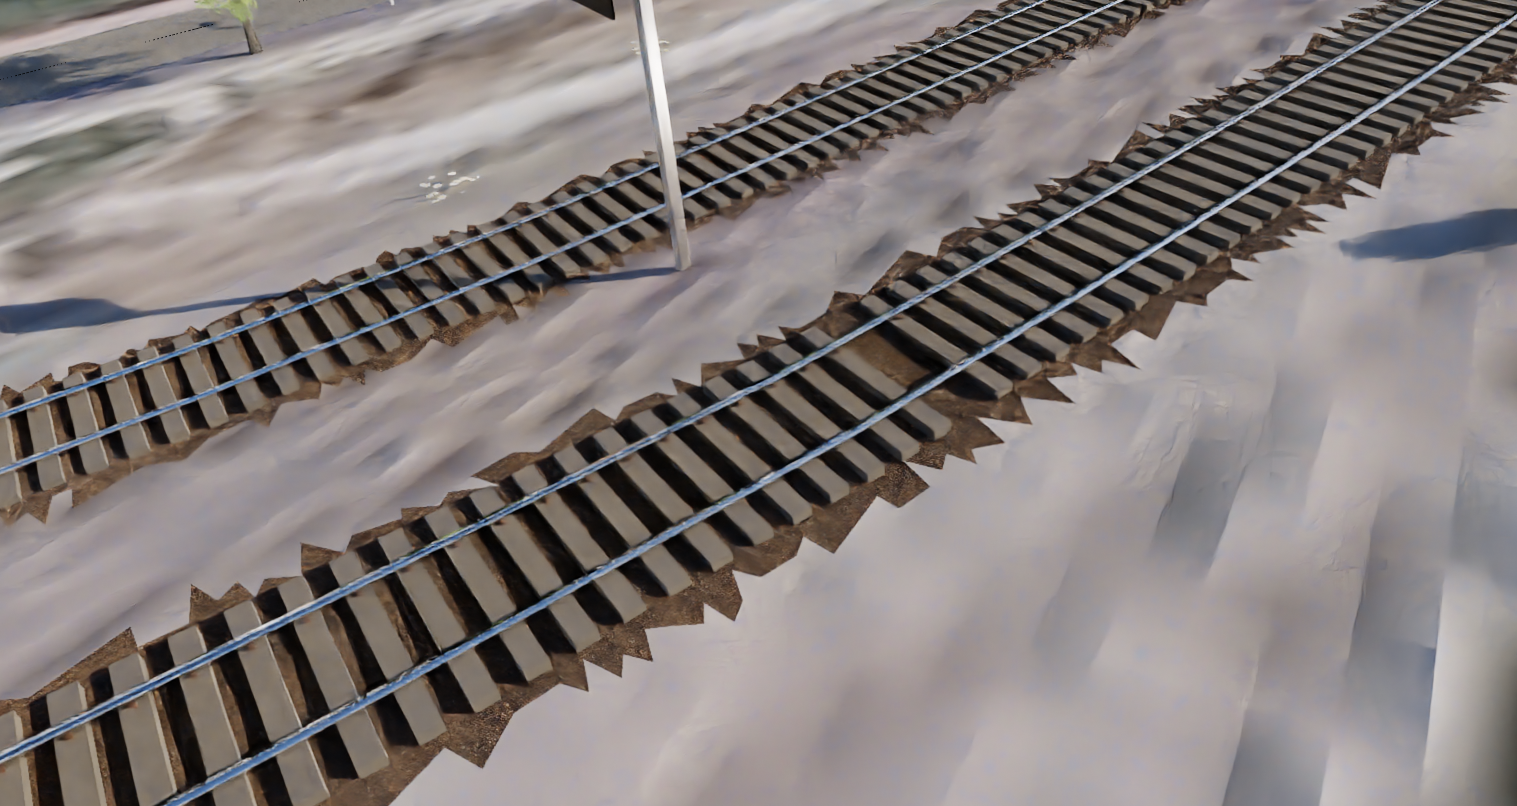
\includegraphics[width=.95\textwidth]{src/img/procedural-tracks/3b-rails-result.png}
    \caption{Rail Tracks - Final Result}
    \label{fig:track-final-result}
\end{figure}

\begin{wrapfigure}{r}{0.3\textwidth}
    \centering
    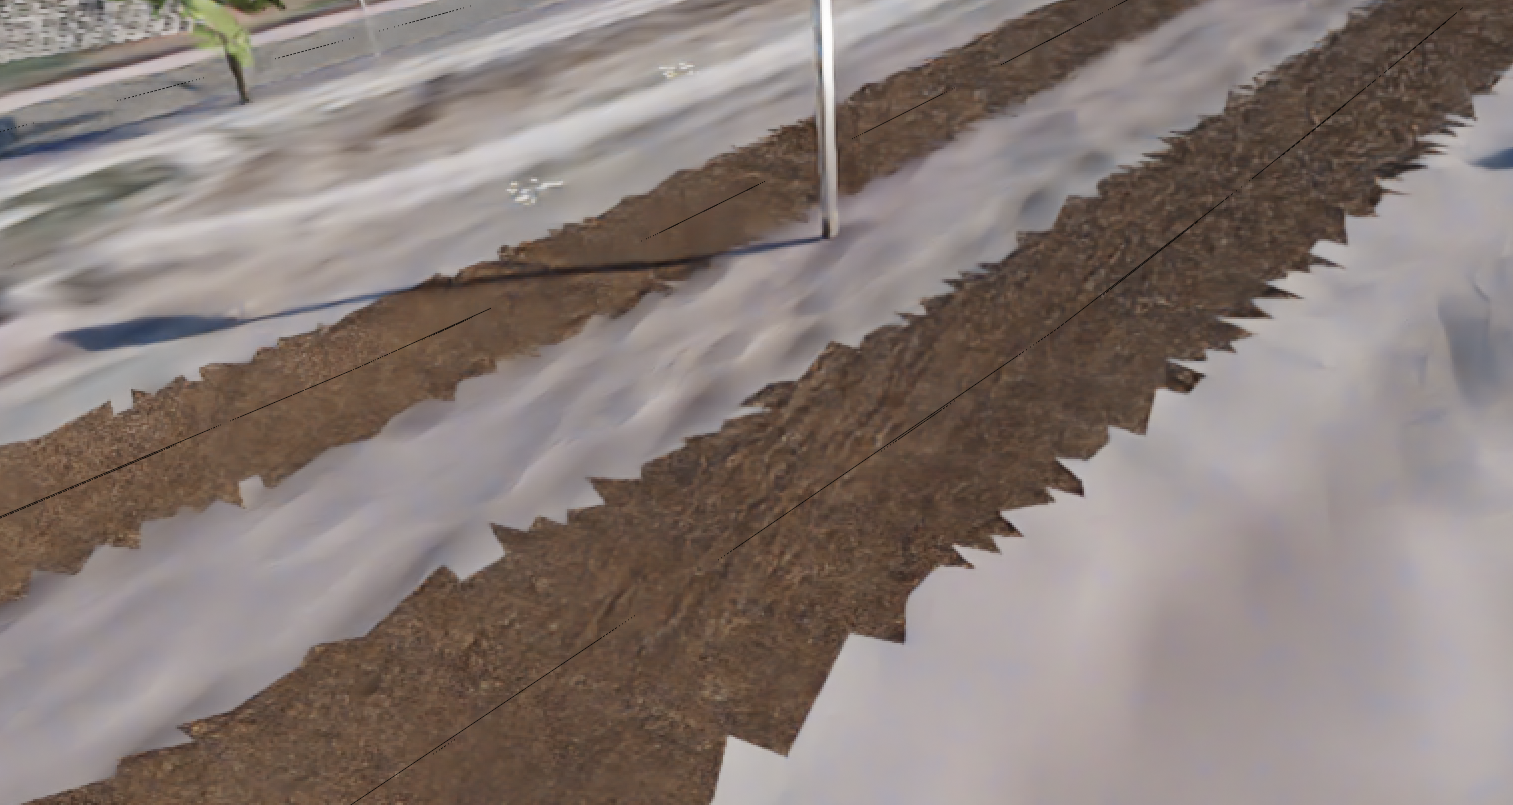
\includegraphics[width=0.28\textwidth]{src/img/procedural-tracks/1-trackbed.png}
    \caption{Track Ballast}
    \label{fig:track-ballast-pic}
\end{wrapfigure}

This section explains in detail the creation of railway objects from the rail track curve. The rail track curve is obtained from OpenStreetMap as described in Section \ref{sec:dowonload-geo-data}, and adjusted to fit the terrain as explained in Section \ref{sec:combine-levels-of-detail}.


First, the ground material immediately around the track is changed into a rock-like texture that represents the track ballast made of crushed stone (Figure \ref{fig:track-ballast-pic}). Then, objects are created using "Geometry Nodes" to procedurally model the metallic rail tracks, the wooden railroad ties, and the rusted metallic bolts that keep them together. The final result is shown in Figure \ref{fig:track-final-result}.

\begin{wrapfigure}{r}{0.3\textwidth}
    \centering
    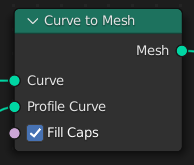
\includegraphics[width=0.28\textwidth]{src/img/procedural-tracks/3a-rails-curve-to-mesh.png}
    \caption{"Curve to Mesh" Geometry Primitive}
    \label{fig:track-curve-to-mesh-primitive}
\end{wrapfigure}




The metallic rails are generated by using the "Curve to Mesh" primitive (Figure \ref{fig:track-curve-to-mesh-primitive}) to enwrap a profile curve over the track path. The profile curve is created by duplicating a small square to the left and right of the origin, to obtain the standard Romanian rail gauge of 1435 mm. A metallic material is set on the rail tracks geometry, with high Specular and Metallic factors.



To aid in creating the "rail-to-rail" segmentation mask used in the machine learning model from Chapter \ref{chapter:testing-and-evaluation}, we also create a transparent placeholder volume between the tracks. This volume is part of the track object, but does not appear in the rendered image. The placeholder volume is shown in Figure \ref{fig:track-transparent-segmentation-placeholder}.


\begin{wrapfigure}{r}{0.3\textwidth}
    \centering
    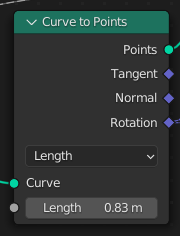
\includegraphics[width=0.28\textwidth]{src/img/procedural-tracks/2c-planks-curve-to-points.png}
     \caption{"Curve to Points" Geometry Primitive}
     \label{fig:curve-to-points}
\end{wrapfigure}

The wooden railroad ties (traverse planks) are similarly generated using only the railway curve. First, the wooden plank geometry is generated by scaling a cube to the standard wooden railroad tie size of 2600 mm×160 mm×220 mm. The planks are then instanced along the rail track curve, using the "Curve to Points" geometry primitive (Figure \ref{fig:curve-to-points}. Additionally, on each plank, we add two rust-colored hexagonal bolts. The bolts are created by using a Cylinder primitive with a setting of 6 sides, then instanced at the same time as the railroad ties.

\begin{figure}[!htb]
   \begin{minipage}{0.3\textwidth}
     \centering
     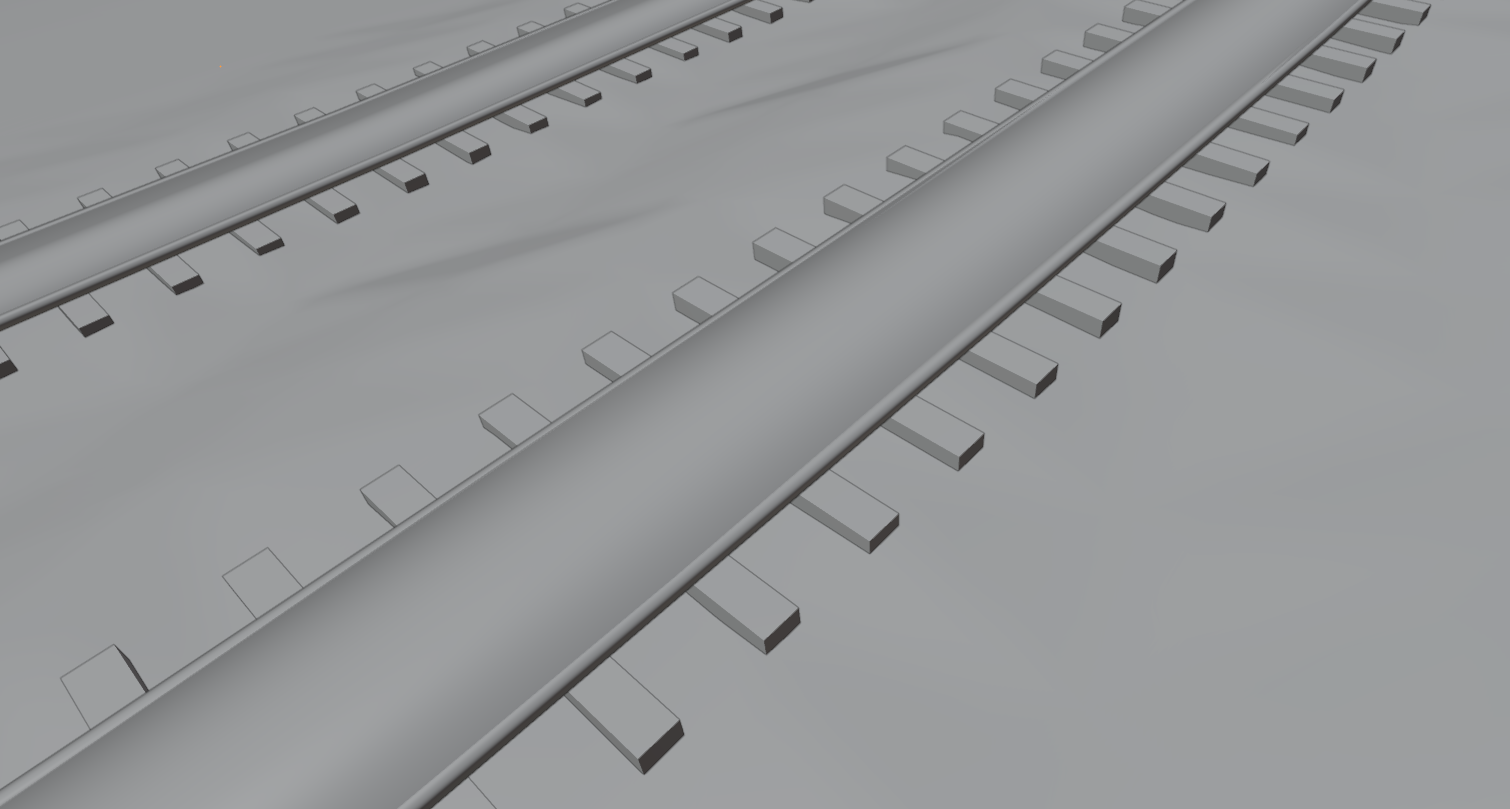
\includegraphics[width=.97\linewidth]{src/img/procedural-tracks/3c-matte-view.png}
     \caption{Transparent Segmentation Placeholder Volume}
     \label{fig:track-transparent-segmentation-placeholder}
   \end{minipage}\hfill
   \begin{minipage}{0.3\textwidth}
     \centering
     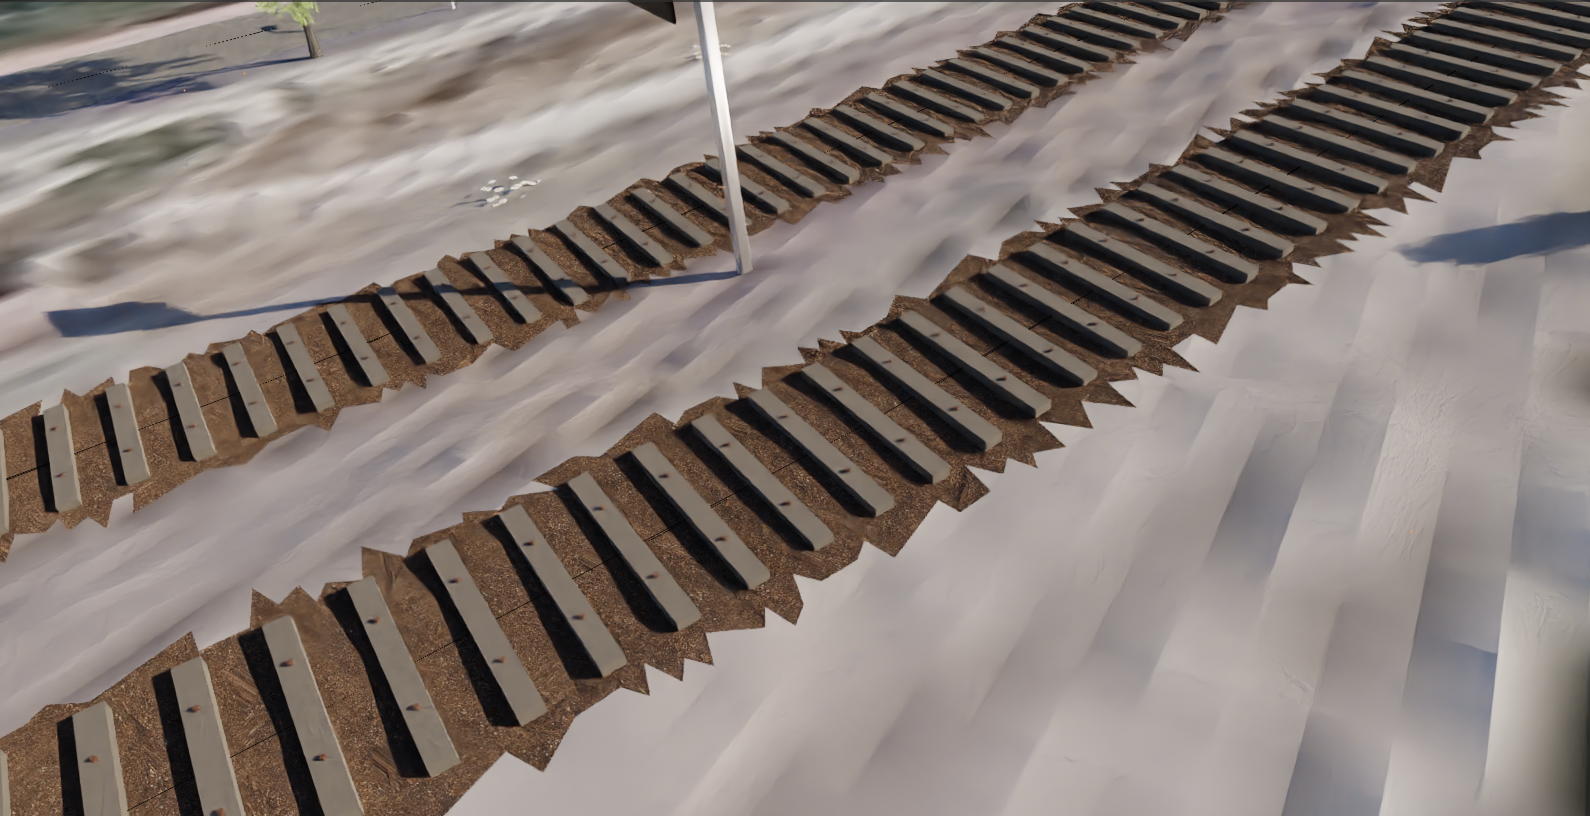
\includegraphics[width=\linewidth]{src/img/procedural-tracks/2b-planks-far.png}
     \caption{Railroad Ties in Far Configuration}
     \label{fig:wood-far}
   \end{minipage}\hfill
   \begin{minipage}{0.3\textwidth}
     \centering
     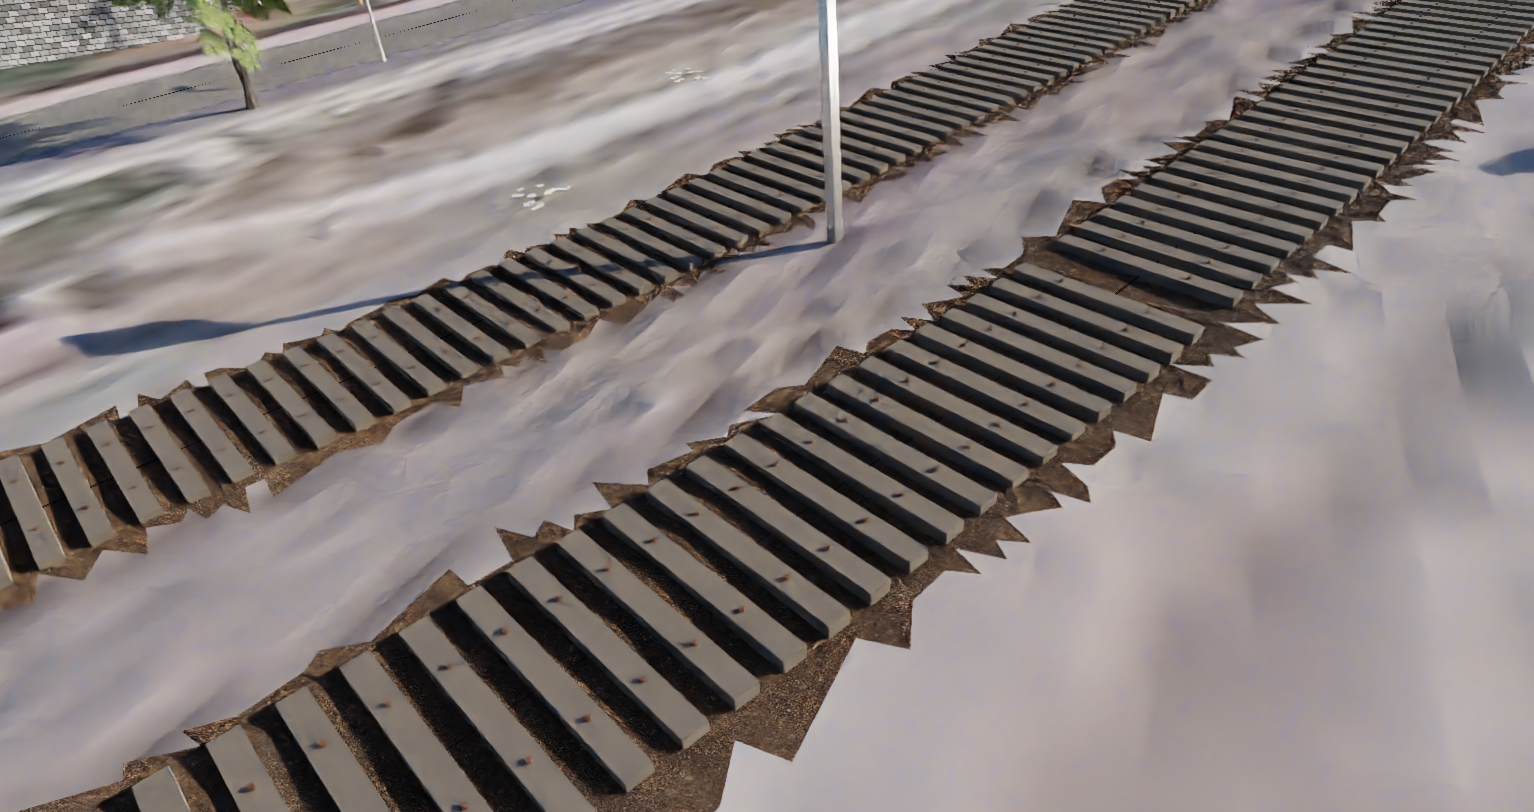
\includegraphics[width=.97\linewidth]{src/img/procedural-tracks/2a-planks-bolts-close.png}
     \caption{Railroad Ties in Close Configuration}
     \label{fig:wood-close}
   \end{minipage}
\end{figure}



Finally, railroad signage is generated by instancing a 3D model from the model library. The signage is placed alongside the tracks, at a set distance from the center.

To reduce the memory usage of the scene generation, only the visible objects are instanced during rendering. This includes rail tracks, ties, bolts, and signs. This is implemented by using ray tracing primitives to create a View Frustum Culling Geometry Node. This node is configured with a slightly larger view cone than the virtual camera, to ensure all objects from the camera are instantiated at the right time, and that objects from slightly outside the camera's view still cast shadows in the scene.


A similar process happens with the generation of Roads: the ground area around the road curves is painted in asphalt material, and power lines are placed along the side of the road. Since the roads in this simulation are designed only as part of the background of the generated railroad footage, we did not implement finer details involving roads, such as parked or moving cars, road signage, semaphores or road barriers. The principles behind implementing these are identical to the railroad generation, and such we leave them as an exercise to the reader.





With the foreground objects finished, the scene generation continues with background details: vegetation and buildings.

% ###############################################################
\section{Vegetation Scatter and Geometry Caching}
\label{sec:vegetation-scatter}

After placing railroads, roads and buildings, we complete the background with instanced 3D objects representing vegetation. The process involves randomly distributing points on the terrain, while ensuring points are placed at adequate distance to roads, rail tracks, and buildings. 

The distances to various terrain features are calculated with a first Geometry Nodes Group and stored in the terrain as Vertex Group metadata called TODO NAME VERTEX GROUP.

TODO blender distance vertex group screenshot

Even through the Blender Geometry Nodes can be used as a functional, unidirectional data flow, it has no support for result caching. This means all Geometry Node logic must execute at every frame of the simulation, which greatly impacts the simulation frame rate. To work around this limitation, we store results of expensive computations in temporary objects, by "applying" the Geometry Nodes Modifier in Blender. This technique is used for vegetation scatter, as distributing tens of thousands of points to anchor vegetation elements is an expensive procedure.

A second Geometry Nodes Group is used to randomly generate points that respect the minimum distance to features. These points are stored in temporary objects, to avoid expensive re-computation at every frame of the render. These temporary objects also store a number of randomly generated attributes alongside the position, such as scale, rotation, and instanced object index. The stored object must be of the "Mesh" Geometry type, as any other type is not saved when the Geometry Node is applied.

Finally, the points are instantiated into randomly selected objects of each vegetation type. The models for the vegetation objects are taken from the 3D model library.


TODO veg geometry screenshot


With the vegetation instantiated, we can start rendering the scene. The rendering loop is described in the next section.

% ###############################################################
\section{Scene Setup and Rendering Loop}
\label{sec:rendering}


First, scene parameter randomization happens, where random default values are set for all parameters. Parameters include both simulation settings (such as render resolution, and output video frames per second), and scene parameters (like cloud density and level, or sky texture sun orientation and strength).

Then, some custom frame setup logic is applied: user logic affects camera position and movement, changes simulation parameters, or adds and removes additional objects from the scene. This is controlled frame by frame, and can optionally sample output images from the render process of the next frame, in order to decide on how to affect the next frame.

TODO render loop / interactive PYTHON API

As a predefined number of frames are rendered, the images and related metadata are stored in the output storage location.
